\documentclass[10pt]{book}
\usepackage[FINAL]{../../../boilerplate/rexx} 
\usepackage{hyperref}
\usepackage{graphics}
\usepackage{geometry}
\usepackage{setspace}
\usepackage{etoolbox}
\usepackage{fontspec}
\usepackage{tocloft}
\usepackage{titlesec}
\setmainfont[Mapping=tex-text]{Georgia Pro}
\setmonofont[Mapping=tex-text,Scale=0.82]{IBM Plex Mono}
\usepackage{tabularx}
\usepackage{booktabs}
\usepackage{makeidx}
\usepackage{color}
\usepackage{xcolor}
\usepackage{listings}

%fancyhdr for page headers, footers, numbers
\usepackage{fancyhdr}

\pagestyle{fancy}
\fancyhf{} % Clear default header/footer settings

\fancyheadoffset{0pt}
\addtolength{\headsep}{15pt}

% Define the headers
\fancyhead[RO]{\normalfont \nouppercase{\rightmark}}  % Chapter title on right pages, aligned right
\fancyhead[LE]{\normalfont \nouppercase{\leftmark}}   % Section title on left pages, aligned right

% Ensure chapter and section marks update correctly
%% \renewcommand{\chaptermark}[1]{\markright{#1}\normalfont \thechapter.\ #1}
%% \renewcommand{\sectionmark}[1]{\markleft{#1}\normalfont \thesection.\ #1}

\fancyfoot[C]{\thepage}

% avoid headers on empty pages
\usepackage{emptypage}

\usepackage{caption}
\usepackage{longtable}
\usepackage{colortbl}
\usepackage{framed}
\usepackage{fancyvrb}
\definecolor{shadecolor}{rgb}{0.9,0.9,0.9}
\definecolor{nrblue}{RGB}{38,139,210}
\definecolor{nrgreen}{RGB}{65,133,153}
\definecolor{nrcyan}{RGB}{42,161,152 }
\definecolor{nrorange}{RGB}{203 ,75,22}
\definecolor{nrgrey}{RGB}{101,123,131}
\usepackage{alltt}
%% \DeclareCaptionFont{white}{\color{white}}
%% \DeclareCaptionFormat{listing}{\colorbox{gray}{\parbox{\textwidth}{#1#2#3}}}
%% \captionsetup[lstlisting]{format=listing,labelfont=white,textfont=white}
\usepackage[official]{eurosym}
%% \makeatletter
%% \@empty\z@\@empty
%% \lst@CCPutMacro\lst@ProcessOther {"2D}{\lst@ttfamily{-{}}{-{}}} 
%% \makeatother
%%\renewcommand*\familydefault{\sfdefault}

\lstdefinelanguage{NetRexx}
{morekeywords={abstract,adapter,binary,case,catch,class,constant,dependent,deprecated,digits,do,else,end,engineering,extends,final,finally,for,forever,if,implements,indirect,import,indirect,inheritable,interface,iterate,label,leave,loop,method,native,nop,numeric,options,otherwise,over,package,parent,parse,private,properties,protect,public,return,returns,rexx,say,scientific,set,digits,form,select,shared,signal,signals,sourceline,static,super,then,this,until,used,upper,volatile,when,where,while},
sensitive=false,
extendedchars=true,
morecomment=[s]={/*}{*/},
morecomment=[l]{--},
morecomment=[s]{/**}{*/},
morestring=[b]",
morestring=[d]",
morestring=[b]',
morestring=[d]'}

\lstset{language=NetRexx,
  captionpos=none,
  tabsize=3,
  alsolanguage=Rexx,
  keywordstyle=\color{nrorange},
  commentstyle=\color{nrgrey},
  stringstyle=\color{nrgreen},
  numbers=none,
  numberstyle=\tiny,
  numbersep=5pt,
  breaklines=true,
  showstringspaces=false,
  index=[1][keywords],
  columns=fixed,
  basicstyle=\fontsize{10}{10}\fontspec{Hack},emph={label}
}

%% \lstdefinelanguage
%%    {x64Assembler}     % add a "x64" dialect of Assembler
%%    [x86masm]{Assembler} % based on the "x86masm" dialect
%%    % with these extra keywords:
%%    {morekeywords={CDQE,CQO,CMPSQ,CMPXCHG16B,JRCXZ,LODSQ,MOVSXD, %
%%                   POPFQ,PUSHFQ,SCASQ,STOSQ,IRETQ,RDTSCP,SWAPGS, %
%%                   rax,rdx,rcx,rbx,rsi,rdi,rsp,rbp, %
%%                   r8,r8d,r8w,r8b,r9,r9d,r9w,r9b, %
%%                   r10,r10d,r10w,r10b,r11,r11d,r11w,r11b, %
%%                   r12,r12d,r12w,r12b,r13,r13d,r13w,r13b, %
%%                   r14,r14d,r14w,r14b,r15,r15d,r15w,r15b}} % etc.

%% \lstset{language=x64Assembler}

\lstdefinelanguage
  [x86]{Assembler}%
  {moreemph=[3]{al,ah,ax,eax,bl,bh,bx,ebx,cl,ch,cx,ecx,dl,dh,dx,edx,%
      si,esi,di,edi,bp,ebp,sp,esp,cs,ds,es,ss,fs,gs,cr0,cr1,cr2,cr3,%
      db0,db1,db2,db3,db4,db5,db6,db7,tr0,tr1,tr2,tr3,tr4,tr5,tr6,tr7,%
      st},
   morekeywords=[1]{aaa,aad,aam,aas,adc,add,and,arpl,bound,bsf,bsr,bswap,bt,btc,%
      btr,bts,call,cbw,cdq,clc,cld,cli,clts,cmc,cmp,cmps,cmpsb,cmpsw,%
      cmpsd,cmpxchg,cwd,cwde,daa,das,dec,div,enter,hlt,idiv,imul,in,%
      inc,ins,int,into,invd,invlpg,iret,ja,jae,jb,jbe,jc,jcxz,jecxz,%
      je,jg,jge,jl,jle,jna,jnae,jnb,jnbe,jnc,jne,jng,jnge,jnl,jnle,%
      jno,jnp,jns,jnz,jo,jp,jpe,jpo,js,jz,jmp,lahf,lar,lea,leave,lgdt,%
      lidt,lldt,lmsw,lock,lods,lodsb,lodsw,lodsd,loop,loopz,loopnz,%
      loope,loopne,lds,les,lfs,lgs,lss,lsl,ltr,mov,movs,movsb,movsw,%
      movsd,movsx,movzx,mul,neg,nop,not,or,out,outs,pop,popl,popq,popa,popad,%
      popf,popfd,push,pusha,pushad,pushf,pushfd,rcl,rcr,rep,repe,%
      repne,repz,repnz,ret,retf,rol,ror,sahf,sal,sar,sbb,scas,seta,%
      setae,setb,setbe,setc,sete,setg,setge,setl,setle,setna,setnae,%
      setnb,setnbe,setnc,setne,setng,setnge,setnl,setnle,setno,setnp,%
      setns,setnz,seto,setp,setpe,setpo,sets,setz,sgdt,shl,shld,shr,%
      shrd,sidt,sldt,smsw,stc,std,sti,stos,stosb,stosw,stosd,str,sub,%
      test,testl,testq,verr,verw,wait,wbinvd,xadd,xchg,xlatb,xor,xorl,xorq,fabs,fadd,fbld,%
      fbstp,fchs,fclex,fcom,fcos,fdecstp,fdiv,fdivr,ffree,fiadd,ficom,%
      fidiv,fidivr,fild,fimul,fincstp,finit,fist,fisub,fisubr,fld,fld1,%
      fldl2e,fldl2t,fldlg2,fldln2,fldpi,fldz,fldcw,fldenv,fmul,fnop,%
      fpatan,fprem,fprem1,fptan,frndint,frstor,fsave,fscale,fsetpm,%
      fsin,fsincos,fsqrt,fst,fstcw,fstenv,fstsw,fsub,fsubr,ftst,fucom,%
      fwait,fxam,fxch,fxtract,fyl2x,fyl2xp1,f2xm1},%
   morekeywords=[2]{.align,.alpha,assume,byte,code,comm,comment,.const,%
      .cref,.data,.data?,db,dd,df,dosseg,dq,dt,dw,dword,else,end,endif,%
      endm,endp,ends,eq,equ,.err,.err1,.err2,.errb,.errdef,.errdif,%
      .erre,.erridn,.errnb,.errndef,.errnz,event,exitm,extrn,far,%
      .fardata,.fardata?,function,fword,ge,group,gt,high,if,if1,if2,ifb,ifdef,%
      ifdif,ife,ifidn,ifnb,ifndef,include,includelib,irp,irpc,label,%
      .lall,le,length,.lfcond,.list,local,low,lt,macro,mask,mod,.model,%
      name,ne,near,offset,org,out,page,proc,ptr,public,purge,qword,.%
      radix,record,rept,.sall,seg,segment,.seq,.sfcond,short,size,%
      .stack,struc,subttl,tbyte,.tfcond,this,title,type,.type,width,%
      word,.xall,.xcref,.xlist},%
   alsoletter=.,alsodigit=?,alsodigit=\$,%
   otherkeywords={\%,\$,@},%
   sensitive=f,%
   morestring=[b]",%
   morestring=[b]',%
   morecomment=[l];%
   morecomment=[l]##,%
   }[keywords,comments,strings,emph]

\lstdefinelanguage
   [x86_64]{Assembler}     % add a "x86_64" dialect of Assembler
   [x86]{Assembler}        % based on the "x86" dialect
   % with these extra keywords:
   {morekeywords={cdqe,cqo,cmpsq,cmpxchg16b,jrcxz,lodsq,movsxd, %
                  popfq,pushfq,scasq,stosq,iretq,rdtscp,swapgs, %
                  movl,movq,pushl,pushq,subl,subq,cmpl,cmpq,    %
                  addl,addq,incl,incq,leal,leaq,                %
                  vmovsd, vaddsd, vsubsd, vmulsd, vdivsd,       %
                  vfmadd132sd,vfmadd213sd,vfmadd231sd,          %
                },                                   %
   moreemph=[3]{rax,rdx,rcx,rbx,rsi,rdi,rsp,rbp,rip, %
                r8,r8d,r8w,r8b,r9,r9d,r9w,r9b,       %
                r10,r10d,r10w,r10b,r11,r11d,r11w,r11b,%
                r12,r12d,r12w,r12b,r13,r13d,r13w,r13b,%
                r14,r14d,r14w,r14b,r15,r15d,r15w,r15b,%
      xmm0, xmm1, xmm2, xmm3, xmm4, xmm5, xmm6, xmm7,%
      ymm0, ymm1, ymm2, ymm3, ymm4, ymm5, ymm6, ymm7,%
    }} % etc.


\lstdefinelanguage
   {zAssembler}     % add a s390 dialect of Assembler
   [x86masm]{Assembler} 
   % with these extra keywords:
   {morekeywords={PRINT,GEN,END,LTORG,AMODE,RMODE,USING
                 }}

\lstset{language=zAssembler,
  tabsize=3,
  alsolanguage=rexx,
  keywordstyle=\color{blue},
  commentstyle=\color{nrgrey},
  stringstyle=\color{nrgreen},
  numbers=left,
  numberstyle=\tiny,
  numbersep=5pt,
  numberbychapter=false,
  breaklines=true,
  showstringspaces=false,
  index=[1][keywords],
  columns=fixed,
  basicstyle=\fontsize{9}{9}\fontspec{JuliaMono},emph={label}
}



% MIPS Assembly language definition for the LaTeX `listings' package
%
% The list of instructions and directives are those understood by the
% MARS MIPS Simulator [http://courses.missouristate.edu/KenVollmar/MARS/]
%
% Author: Eric Walkingshaw <eric@walkingshaw.net>
%
% This code is in the public domain.
%
% Here is an example style. I like it for slides, but you might want 
% something a bit less noisy for print. :)
%
% \definecolor{CommentGreen}{rgb}{0,.6,0}
% \lstset{
%   language=[mips]Assembler,
%   escapechar=@, % include LaTeX code between `@' characters
%   keepspaces,   % needed to preserve spacing with lstinline
%   basicstyle=\footnotesize\ttfamily\bfseries,
%   commentstyle=\color{CommentGreen},
%   stringstyle=\color{cyan},
%   showstringspaces=false,
%   keywordstyle=[1]\color{blue},    % instructions
%   keywordstyle=[2]\color{magenta}, % directives
%   keywordstyle=[3]\color{red},     % registers
% }

%% \ProvidesPackage{mips}

%% \RequirePackage{listings}

\lstdefinelanguage[mips]{Assembler}{%
  % so listings can detect directives and register names
  alsoletter={.\$},
  % strings, characters, and comments
  morestring=[b]",
  morestring=[b]',
  morecomment=[l]\#,
  % instructions
  morekeywords={[1]abs,abs.d,abs.s,add,add.d,add.s,addi,addiu,addu,%
    and,andi,b,bc1f,bc1t,beq,beqz,bge,bgeu,bgez,bgezal,bgt,bgtu,%
    bgtz,ble,bleu,blez,blt,bltu,bltz,bltzal,bne,bnez,break,c.eq.d,%
    c.eq.s,c.le.d,c.le.s,c.lt.d,c.lt.s,ceil.w.d,ceil.w.s,clo,clz,%
    cvt.d.s,cvt.d.w,cvt.s.d,cvt.s.w,cvt.w.d,cvt.w.s,div,div.d,div.s,%
    divu,eret,floor.w.d,floor.w.s,j,jal,jalr,jr,l.d,l.s,la,lb,lbu,%
    ld,ldc1,lh,lhu,li,ll,lui,lw,lwc1,lwl,lwr,madd,maddu,mfc0,mfc1,%
    mfc1.d,mfhi,mflo,mov.d,mov.s,move,movf,movf.d,movf.s,movn,movn.d,%
    movn.s,movt,movt.d,movt.s,movz,movz.d,movz.s,msub,msubu,mtc0,mtc1,%
    mtc1.d,mthi,mtlo,mul,mul.d,mul.s,mulo,mulou,mult,multu,mulu,neg,%
    neg.d,neg.s,negu,nop,nor,not,or,ori,rem,remu,rol,ror,round.w.d,%
    round.w.s,s.d,s.s,sb,sc,sd,sdc1,seq,sge,sgeu,sgt,sgtu,sh,sle,%
    sleu,sll,sllv,slt,slti,sltiu,sltu,sne,sqrt.d,sqrt.s,sra,srav,srl,%
    srlv,sub,sub.d,sub.s,subi,subiu,subu,sw,swc1,swl,swr,syscall,teq,%
    teqi,tge,tgei,tgeiu,tgeu,tlt,tlti,tltiu,tltu,tne,tnei,trunc.w.d,%
    trunc.w.s,ulh,ulhu,ulw,ush,usw,xor,xori},
  % assembler directives
  morekeywords={[2].align,.ascii,.asciiz,.byte,.data,.double,.extern,%
    .float,.globl,.half,.kdata,.ktext,.set,.space,.text,.word},
  % register names
  morekeywords={[3]\$0,\$1,\$2,\$3,\$4,\$5,\$6,\$7,\$8,\$9,\$10,\$11,%
    \$12,\$13,\$14,\$15,\$16,\$17,\$18,\$19,\$20,\$21,\$22,\$23,\$24,%
    \$25,\$26,\$27,\$28,\$29,\$30,\$31,%
    \$zero,\$at,\$v0,\$v1,\$a0,\$a1,\$a2,\$a3,\$t0,\$t1,\$t2,\$t3,\$t4,
    \$t5,\$t6,\$t7,\$s0,\$s1,\$s2,\$s3,\$s4,\$s5,\$s6,\$s7,\$t8,\$t9,%
    \$k0,\$k1,\$gp,\$sp,\$fp,\$ra},
}[strings,comments,keywords]

\lstdefinelanguage{rxas}
{morekeywords={
appendchar,
addf,
addi,
addi,
amap,
amap,
and,
append,
addf,
bcf,
bcf,
bct,
bct,
bctnm,
bctnm,
beq,
bge,
bge,
bgt,
bgt,
ble,
ble,
blt,
blt,
bne,
bne,
bpoff,
bpon,
br,
brf,
brt,
brtpandt,
beq,
brtpt,
brtf,
call,
cnop,
call,
concchar,
concat,
concat,
concat,
call,
copy,
divf,
dec,
dec0,
dcall,
dec2,
dec1,
divf,
divi,
divi,
dllparms,
dropchar,
divf,
exit,
exit,
exit,
fadd,
fadd,
fcopy,
fdiv,
fdiv,
fdiv,
feq,
fformat,
fgt,
fgt,
fgt,
fgte,
fgte,
fgte,
flt,
flt,
flt,
flte,
flte,
flte,
fmult,
fmult,
fndblnk,
fndnblnk,
fne,
fne,
fpow,
fpow,
fsex,
fsub,
fsub,
fsub,
ftob,
ftoi,
ftos,
feq,
getstrpos,
gmap,
gettp,
gmap,
getbyte,
hexchar,
iadd,
iadd,
igt,
iand,
icopy,
idiv,
idiv,
idiv,
ieq,
ieq,
igt,
igte,
iand,
igte,
igte,
ilt,
ilt,
ilt,
ilte,
ilte,
ilte,
imod,
imod,
imod,
imult,
imult,
inc,
inc0,
inc1,
ine,
igt,
ine,
inot,
inot,
ior,
ior,
ipow,
ipow,
ipow,
irand,
irand,
isex,
ishl,
ishl,
ishr,
ishr,
isub,
isub,
isub,
itof,
itos,
ixor,
ixor,
inc2,
linkattr,
load,
linkattr,
loadsettp,
load,
load,
load,
link,
loadsettp,
loadsettp,
metaloadedmodules,
map,
map,
metadecodeinst,
metaloadcalleraddr,
metaloaddata,
metaloadedprocs,
metaloadfoperand,
metaloadinst,
metaloadioperand,
metaloadmodule,
metaloadpoperand,
metaloadsoperand,
move,
mtime,
multf,
multi,
metalinkpreg,
multi,
multf,
nsmap,
nsmap,
nsmap,
null,
nsmap,
not,
opendll,
or,
padstr,
pmap,
pmap,
poschar,
ret,
ret,
ret,
ret,
ret,
ret,
rseq,
rseq,
readline,
sappend,
say,
say,
say,
say,
sayx,
sayx,
sconcat,
sconcat,
sconcat,
scopy,
seq,
seq,
setortp,
setstrpos,
settp,
sgt,
sgt,
sgt,
sgte,
sgte,
sgte,
slt,
slt,
slt,
slte,
slte,
slte,
sne,
sne,
stof,
stoi,
strchar,
strchar,
strlen,
strlower,
strupper,
subf,
subf,
subf,
subi,
subi,
substcut,
substr,
substring,
swap,
say,
time,
transchar,
triml,
triml,
trimr,
trimr,
trunc,
trunc,
unlink,
unmap,
xtime,
  },
sensitive=false,
extendedchars=true,
morecomment=[s]={/*}{*/},
morecomment=[l]{*},
morecomment=[s]{/**}{*/},
morestring=[b]",
morestring=[d]",
morestring=[b]',
morestring=[d]'}

\lstset{language=rxas,
  captionpos=none,
  tabsize=3,
  keywordstyle=\color{nrorange},
  commentstyle=\color{nrgrey},
  stringstyle=\color{nrgreen},
  numbers=left,
  numberstyle=\tiny,
  numbersep=5pt,
  breaklines=true,
  showstringspaces=false,
  index=[1][keywords],
  columns=fixed,
  basicstyle=\fontsize{10}{10}\fontspec{Hack},emph={label}
}

%% \input{../../../boilerplate/jclformat}
\usepackage{pst-barcode,pstricks-add}
\usepackage{bashful}
\usepackage{metalogo}
\usepackage{marginnote}
\usepackage{pdfpages}
\usepackage{svg}
\usepackage{float}
\makeindex
\DeclareGraphicsExtensions{.jpg,.png}
\setlength{\parskip}{8pt}
\setlength{\parindent}{0pt}
\usepackage{enumitem}
\usepackage{underscore}
\usepackage{babel}
\usepackage{graphicx}
\usepackage{array}
% \usepackage{tabularx}
\usepackage{multirow}
\usepackage{threeparttable}
\usepackage{longtable}
\usepackage{booktabs}
\usepackage{makeidx}
\usepackage{framed}
\usepackage{alltt}
\usepackage{barracuda}
\usepackage{longtable}
\usepackage{graphicx}
\usepackage{wrapfig}
\usepackage{multicol}
\usepackage[CJK]{ucharclasses}
\usepackage[comma]{natbib}           % CSLI Pubs favored bibliography package.
%% \bibliographystyle{cslipubs-natbib}  % CSLI Pubs bibliography format.
\bibliographystyle{plainnat}  % CSLI Pubs bibliography format.
% defines for consistent use
\newcommand{\crexx}{\textsc{crexx}}
\newcommand{\rexx}{R\textsc{exx}}
%% \newcommand{\nr}{Net\textsc{rexx}}
%% \newcommand{\nrpackagename}{\splice{java GetPackageName}}
%% \newcommand{\minimalJVMversion}{8}
%% \newcommand{\maximalJVMversion}{19ea}
\newcommand{\keyword}[1]{\texttt{#1}}
\newcommand{\code}[1]{\texttt{#1}}
%% \newcommand{\thisyear}{\splice{java TexYear}}
\newcommand{\tightlist}{}
\newcommand{\Shaded}{\shaded}
\newcommand{\msd}[1]{\msdhelper#1\relax}
\newcommand{\msdhelper}[1]
  {\ifx\relax#1\else
    \ifx-#1--{}\else#1\fi
    \expandafter\msdhelper\fi}
  \newcommand{\doublehyphen}{\mbox{\msd{``-~-''}}}
  \newcommand{\doublehyphenunquoted}{\mbox{\msd{-~-}}}

\newcommand{\simularelease}{12.00, date of release  9 aug 1985}
%% This books starts at chapter 0  
\setcounter{chapter}{-1}
%% the font used for tables
\AtBeginEnvironment{longtable}{\fontspec{1403 Vintage Mono Pro}\small}

%% \setlength{\labelsep}{2em} % Distance between label and text
\setlength{\labelwidth}{75pt} % Width of the label box  

\setlist[description]{font=\normalfont}

\usepackage{sectsty}
%% \partfont{\color{nrgreen}}
\chapterfont{\fontspec{Avenir Light}}
\sectionfont{\fontspec{Avenir Light}}
\subsectionfont{\fontspec{Avenir Light}}
\subsubsectionfont{\fontspec{Avenir Light}}

\usepackage[Sonny]{fncychap}

\raggedbottom

\geometry{left=1in, top=1in, bottom=1in, right=1in}
\setstretch{1.2}
\titlespacing*{\section}{0pt}{*1.5}{*0.5}
\titlespacing*{\subsection}{0pt}{*1.2}{*0.4}

\setlength{\parskip}{0.5em}
\raggedbottom

\makeatletter
\patchcmd{\@startsection}{\@afterindenttrue}{\@afterindentfalse}{}{}
\makeatother

%% heading number left overhang
\makeatletter
\def\@seccntformat#1{\protect\makebox[0pt][r]{\csname
the#1\endcsname\quad}}
\makeatother

%% use the heading fonts in the TOC
%% \renewcommand{\cftsecfont}{\sffamily\bfseries} % Matches section font
%% \renewcommand{\cftsubsecfont}{\sffamily} % Example for subsections

\renewcommand{\cftpartfont}{\sffamily}
\renewcommand{\cftchapfont}{\sffamily} % Matches section font
\renewcommand{\cftchappagefont}{\sffamily} % Matches section font
\renewcommand{\cftsubsecfont}{\sffamily} % Example for subsections
\renewcommand{\cftsubsubsecfont}{\sffamily} % Example for subsections
\renewcommand{\cftsecfont}{\sffamily} % Matches section font

\titleformat{name=\chapter,numberless}[display]
  %{\fontspec{Avenir Light}\filcenter} % formatting applied to the
  % heading text
    {\filcenter} % formatting applied to the heading text
  {}
  {0pt}
  %% {\titlerule \vspace{1ex} \fontspec{Avenir Light} } 
 {\titlerule \vspace{1ex} }  % code before the heading text

\titlespacing*{name=\chapter,numberless}
  {0pt}{-1cm}{1cm}  % left, before, after

  \renewcommand{\contentsname}{\fontspec{Avenir Light}Contents}
  \renewcommand{\indexname}{\fontspec{Avenir Light}Index}
  \renewcommand{\listtablename}{\fontspec{Avenir Light}List of tables}
  \renewcommand{\listfigurename}{\fontspec{Avenir Light}List of figures}
  
  \sectionfont{%
    \hrule                % place a horizontal line
    \vspace{1ex}%         % add some vertical space
    \fontspec{Avenir Light}       % set section title size & style
  }


  


\begin{document}
\renewcommand{\isbn}{978-90-819090-1-3}
\setcounter{tocdepth}{1}
\title{\fontspec{TeX Gyre
    Pagella}\textsc{crexx}\protect\fontspec{Bodoni URW
    Light}\\Application Programming Guide}

\author{The \crexx{} team}
%\date{\null\hfill Version \splice{java org.netrexx.process.NrVersion} of \today}
\date{\null\hfill \today}
\maketitle
\pagenumbering{Roman}
\pagestyle{plain}
\frontmatter
\pagenumbering{Roman}
\pagestyle{plain}
\section*{Publication Data}
\textcopyright  Copyright The Rexx Language Association, 2020 -\splice{crexx TexYear}
%\\

All original material in this publication is published under the Creative Commons - Share Alike 3.0 License as stated at \url{http://creativecommons.org/licenses/by-nc-sa/3.0/us/legalcode}.\\[0.5cm]
The responsible publisher of this edition is identified as \emph{IBizz IT Services and Consultancy}, Amsteldijk 14, 1074 HR Amsterdam, a registered company governed by the laws of the Kingdom of The Netherlands.\\[1cm]
This edition is registered under ISBN \isbn \\[1cm]
\psset{unit=1in}
\begin{pspicture}(3.5,1in)
  \psbarcode{\isbn}{includetext guardwhitespace}{isbn}
\end{pspicture}
\newpage
%%% Local Variables:
%%% mode: latex
%%% TeX-master: t
%%% End:

\tableofcontents

\newpage
\pagenumbering{arabic}
\frontmatter
\large
\chapter{The \crexx{} Programming Series}
This book is part of a library, the \emph{\crexx{} Programming Series}, documenting the \crexx{} programming language and its use and applications. This section lists the other publications in this series, and their roles. These books can be ordered in convenient hardcopy and electronic formats from the Rexx Language Association.
\newline
\newline
\begin{tabularx}{\textwidth}{>{\bfseries}lX}
\toprule
Application Programming Guide & The Application Programming Guide
explains the working of the tools and has examples for building
programs on the platforms it supports.
\\\midrule
Language Reference & Referred to as the CRL, this is meant as the formal definition for the language, documenting its syntax and semantics, and prescribing minimal functionality for language implementers.
\\\midrule
The \crexx{} VM Specification & The \crexx{} VM
Specification, documents the \crexx{} Assembly Language and its execution
by the \crexx{} Virtual Machine. It also contains low level virtual
machine and ABI specifications.
\\\bottomrule
\end{tabularx}
%%% Local Variables: 
%%% mode: latex
%%% TeX-master: t
%%% End: 

\chapter{Typographical conventions}
In general, the following conventions have  been observed in the \crexx{} publications:
\begin{itemize}
\item Body text is in this font
\item Examples of language statements are in a \keyword{keyword} or \textbf{bold} type
\item Variables or strings as mentioned in source code, or things that appear on the console, are in a \texttt{typewriter} type
\item Items that are introduced, or emphasized, are in an \emph{italic} type
\item Included program fragments are listed in this fashion:
\begin{lstlisting}[label=example,caption=Example Listing]
-- salute the reader
say 'hello reader'
\end{lstlisting}
\end{itemize}
The small numbers in the left margin of the listing are meant for easy
reference to the source lines, and are not part of the program.
%%% Local Variables: 
%%% mode: latex
%%% TeX-master: t
%%% End: 


\mainmatter
\def\tightlist{}


\chapter*{About This Book}
The \crexx{} language is a further development, and variant of the
\textsc{Rexx} language\footnote{Cowlishaw, 1979}. This book aims to
document the workings of this implementation and serves as reference
for users and implementors alike.


\section*{History}

\begin{description}
\item[mvp] This version documents the Minimally Viable Product
  release, Q1 2022 and is intended for developers only. It documents
  the RXAS instruction set and \crexx{} level B, which is a typed
  subset of Classic Rexx.
\item[f0047] First version, Git feature [F0047]
\end{description}


\part{Guide}
\chapter{Overview of the toolchain}
In the binary distribution of \crexx{} for your platform, the main
toolchain and a number of utilities are included; all programs are statically linked into
their own executable, and no shared object libraries or dll's are needed.\newline
\begin{wrapfigure}{l}{0.4\textwidth}
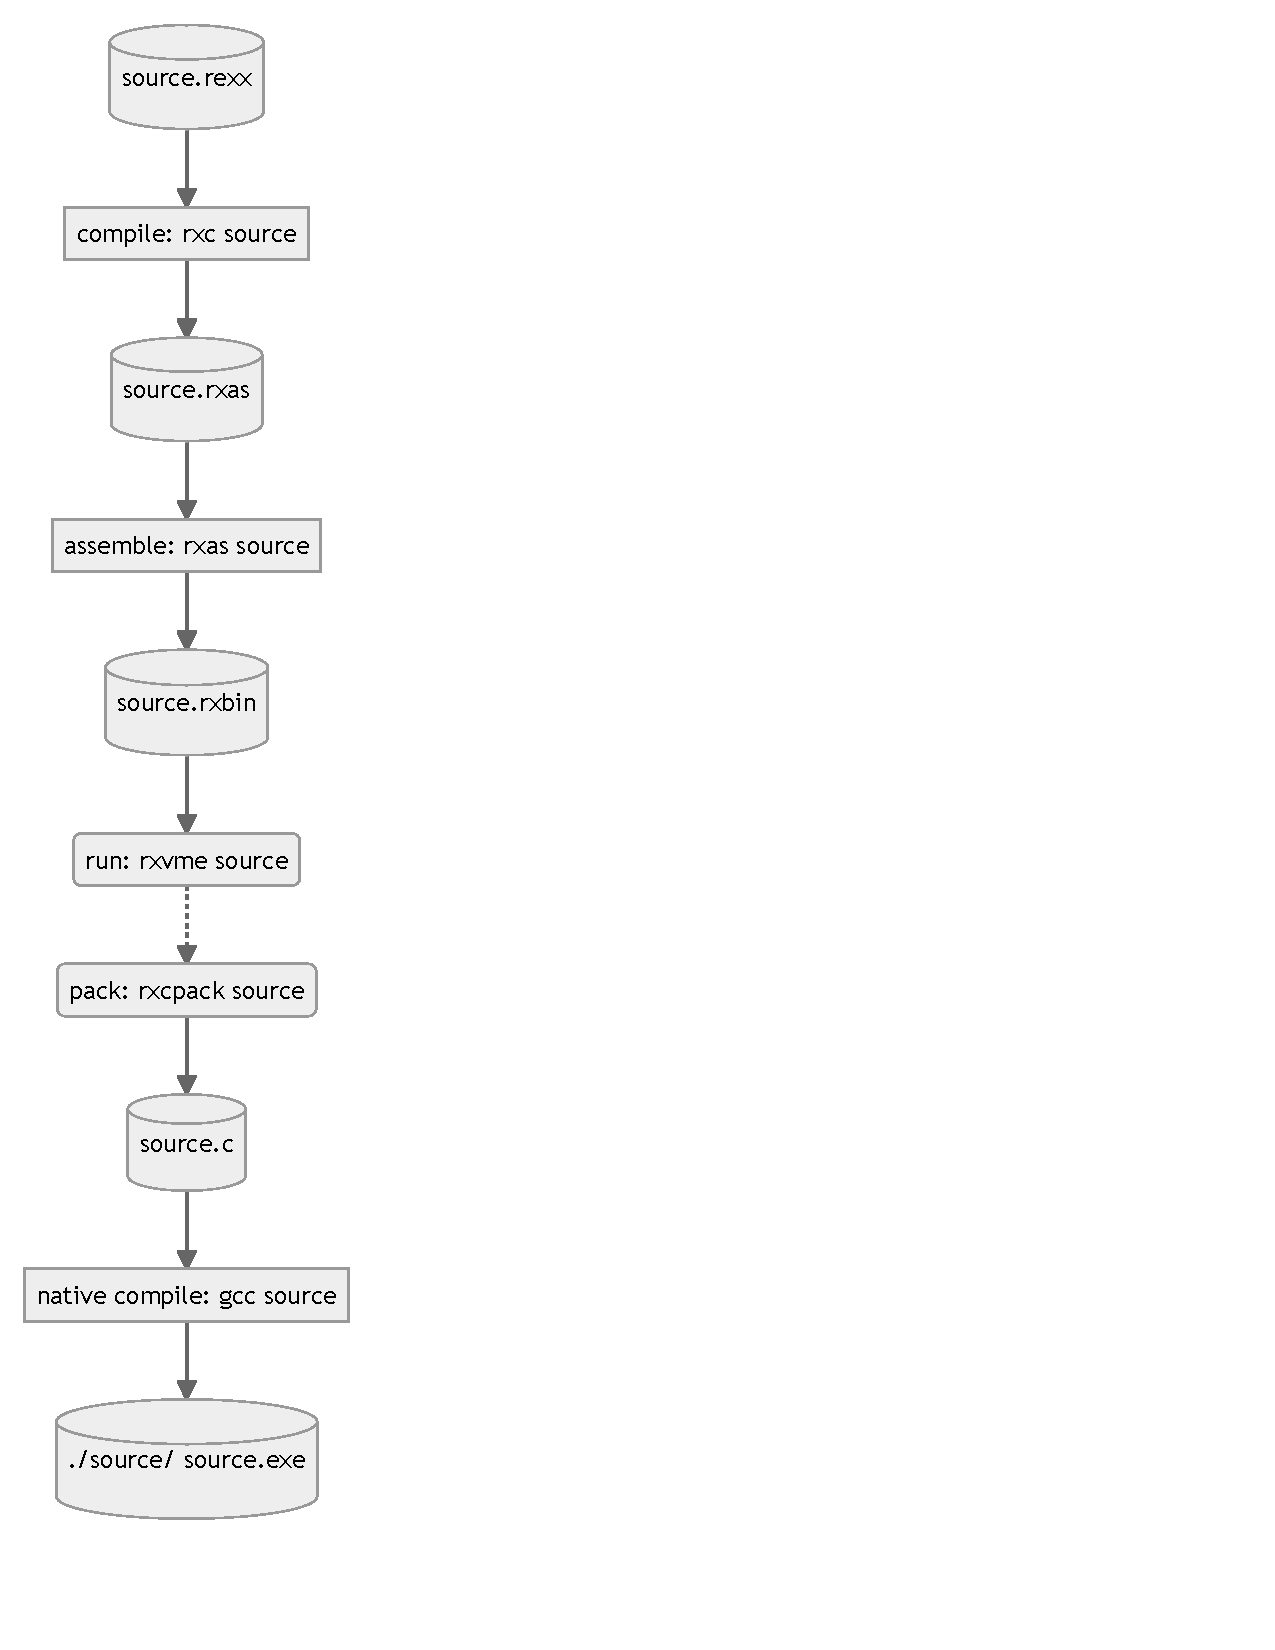
\includegraphics[scale=0.6]{charts/buildflow.pdf}
\end{wrapfigure}
\fussy
Source can be edited with any text editor\footnote{Vi, Emacs, Xedit,
  VS Code, CLion, Eclipse, etc.} of your liking. The sourcefile needs to have an
file extension of \code{.rexx} and contains (Unicode, UTF-8) text. The \code{rxc} \crexx{} compiler
produces a text file which will have a file extension of
\code{.rxas}. The next file in this sequence is produced by the
\code{rxas} assembler and is a binary \code{.rxbin} file. This file is
executable by the \crexx{} \code{rxvme} virtual machine.\newline\newline
\fussy
If you choose to compile a series of \code{*.rxbin} files to a native
executable, the \code{rxcpack} program produces a \code{.c} file,
which can be compiled by any C compiler toolchain.\newline\newline
\fussy
In the following chapters the detailed workflow for the supported platforms is documented.\newline

\chapter{Running \crexx{} on Linux and macOS}
Linux and other Unix-like operating systems like Apple macOS behave in
an identical way when compiling, linking and running a \crexx{}
program.
\hypertarget{running-crexx-entails-compiling}{%
\section{Running cRexx entails
compiling}\label{running-crexx-entails-compiling}}

All Rexx scripts you run with cRexx are compiled by \texttt{rxc} into
Rexx assembler code (.rxas) and then assembled into an .rxbin file,
which contains the Rexx bytecode for execution by the Rexx Virtual
Machine \texttt{rxvm}. During both the compliation and assembler steps
optimization of the code takes place. The rxvm executable takes care of
linking separately compiled modules together and executing them, so one
function can find another.

\hypertarget{a-first-program---hello-world}{%
\section{A first program - Hello
World}\label{a-first-program---hello-world}}

Let's say you have a Rexx exec you would like to run. To not have any
surprises, it is of the \emph{hello world} kind. We have a file called
hello.rexx, containing:

\lstinputlisting[language=rexx,label=hello_example]{examples/hello.rexx}
\fontspec{IBM Plex Mono}
\splice{rxc examples/hello}
\splice{rxas examples/hello}
\begin{shaded}
  \small
\obeylines \splice{rxvm examples/hello}
\end{shaded}
\fontspec{TeX Gyre Pagella}

When cRexx level `C' (for `Classic') is available, the `options levelb'
(on line 2) statement can be left out; for the moment, level B is all we
have, and the compiler will refuse to compile without it.

With all our cRexx executables on the PATH, we only need to do:

\begin{verbatim}
rxc hello
rxas hello
rxvm hello
\end{verbatim}

to see `hello cRexx world!' on the console, as include above this, run
from the included program. Like all the programs in the \crexx{}
documentation, these programs are compiled and run from the included
source by the process that builds the document.

It might be a good idea to make a shell script to execute these three
programs in succession, and perhaps call it `crexx'. But take into
account that this really is a very simple case, in which no built-in
functions are called. We can have a look at the generated rexx assembler
(hello.rxas) file:

\lstinputlisting[language=rxas,label=hellorxas_example]{examples/hello.rxas}

and you can see here that the compiler actually has generated a `say'
assembler instruction for the Rexx `say' instruction. (Assembler became
a whole lot easier with Rexx assembler.) But we did not yet call any
function.

\hypertarget{using-built-in-functions}{%
\section{Using built-in functions}\label{using-built-in-functions}}

Most Rexx programs use the extremely well designed built-in functions.
Now with these functions written in Rexx, and not hidden in the compiler
somewhere, we must tell it to import those from the library where we put
them earlier during the build process. Let's say we want to add a
display of the current weekday to our hello program. This will now be:

\lstinputlisting[language=rexx,label=hellodateexample]{examples/hellodate.rexx}

Never mind the import statement, which you will not need when cRexx
`Classic' level C is available. But in level B, we need this, because we
need the flexibility it affords our plans for the future. See more
about \code{import} on page \pageref{intraImport}.

We must tell the compiler where to find the signature of the date()
function, so it can check if we call it in the correct way, with the
right parameters. This is done with the -i switch, which points to the
directory containing the library - which is called `library', by the
way.

\begin{verbatim}
rxc -i ~/crexx-build/lib/rxfns hellodate
\end{verbatim}

[todo]
% \splice{rxc -i /Users/apps/crexx_release/lib/rxfns examples/hellodate}
% \splice{rxas examples/hellodate}


The assembler runs unchanged, because it trusts the compiler to have
checked if the called function really sits in that library, and has the
right parameters - the right code to call it has been generated.

\begin{verbatim}
rxas hellodate
\end{verbatim}

To run it, we can employ the \texttt{rxvme} executable - this one is
extended with linked-in versions of all the functions in the library:

\begin{verbatim}
rxvme hellodate
\end{verbatim}

which yields:

\fontspec{IBM Plex Mono}
\begin{shaded}
  \small
\obeylines \splice{rxvme examples/hellodate}
\end{shaded}
\fontspec{TeX Gyre Pagella}

\hypertarget{building-a-standalone-executable}{%
\section{Building a standalone
executable}\label{building-a-standalone-executable}}

It is possible to build a standalone executable of this program. It is
possible to run your compiled Rexx program, e.g.~from a USB stick,
without ever installing crexx, on the same OS and instruction set
architecture.

For this, we need the next set of commands, expressed as a Rexx exec:

\begin{verbatim}
/* rexx compile a rexx exec to a native executable */
/* Classic Rexx and NetRexx compatible             */
crexx_home='~/crexx-build'
if arg='' then do
  say 'exec name expected.'
  exit 99
end
parse arg execName'.'extension
if extension<>'' then say 'filename extension ignored.'
'rxc  -i' crexx_home'/lib/rxfns' execName
'rxas' execName
'rxcpack' execName crexx_home'/lib/rxfns/library'
'gcc -o' execName,
'-lrxvml -lmachine -lavl_tree -lplatform -lm -L',
crexx_home'/interpreter -L'crexx_home'/machine -L',
crexx_home'/avl_tree -L'crexx_home'/platform'  execName'.c'
\end{verbatim}

This exec is delivered in the source tree, bin directory.

The exec works by compiling the Rexx program specified (again without
the .rexx file extension) to an .rxbin Rexx bytecode file, which is then
serialized to a C source file, containing the cRexx Virtual Machine and
the library rxbin files, by the rxcpack command. It is a rather peculiar
looking C source, but nevertheless it will compile to a working
executable, which is done by the last step in the exec, here using the
gcc compiler. And you will be able to run it without the overhead of
checking, compiling, tokenizing to bytecode and linking, so it will be
quite fast:

\begin{verbatim}
hello cRexx world!
today is Saturday
./hello  0.00s user 0.00s system 61% cpu 0.009 total
\end{verbatim}

\chapter{Running \crexx{} on Windows operating systems}
\chapter{Running \crexx{} on VM/370CE}
\chapter{Intralanguage calls}
This chapter discusses calls from one \crexx{} procedure to another,
including the built-in function package. Search order is an
intrinsically related concept: how is the called component found. There
are some differences with Classic Rexx and ooRexx, which can call (and interpret)
external procedures in source. In this respect, \crexx{} behaves like
\nr{}, because a called component needs to be compiled, executable
code; for \nr{} a \code{.class} file and in \crexx{} an \code{.rxbin}
file. Level B introduces a package (module) system where a program can
be part of a package and be imported into calling code.
\section{At compile time}
At compile time, a program uses the \code{CALL} statement, or the
function notation with parentheses (also called round brackets). Going
forward, and moving into object oriented notations for other \rexx{}
variants, the latter is going to gain importance, while the
\code{CALL} statement will be fixed in its current functionality. For
that reason, most examples will be in the function notation.

The compiler needs to verify if it is possible to call the called
code: it must be present in executable form, and it needs to have the right
\emph{signature}\footnote{with signature we mean the combination of
  parameters and return type}. The compiler will not automatically compile a callee
of which the source can be located but the executable form is missing;
existing systems based on interpreters will happily interrupt their
work and tokenize another source file when called; the \crexx{}
\code{rxc} compiler will not.

This implies that there are inherent dependencies to be followed
while building an application system that consists of multiple
modules; this is not different than in other compiled
languages. Building utilities like Make or Ninja can provide these
services, and these can be orchestrated by meta-build tools like
CMake. The \crexx{} toolchain itself is built using CMake and from its
build specification in CMake most of these patterns can be gleaned.

The \textbf{import} statement\label{intraImport} tells the compiler we want to
import functions from a certain package.


\section{At runtime}
\chapter{Interlanguage calls}
A \crexx{} program is able to call programs written in the \textsc{Rexx}
language, but also programs native to the platform, using a number of
calling conventions: \[todo: checkrelease\]
\begin{description}
  \item[Address] the \code{address} statement can use the shell and
    I/O indirection to start native executables and provide input, and
    retrieve the output.
    \item[RexxSaa] the traditional RexxSAA calling convention can be
      used for direct interfaces to executables that are designed to
      function as a Rexx library. In its most simple form, these can
      return \textsc{Rexx} strings to the calling program.
      \item[Generic Call Interface] In this RexxSAA extension, the
      type and length of the parameters can be specified by the
      caller\footnote{Which is considered unsafe but sometimes the
        only possibility for programs not designed to be called by \crexx{}}.
    \end{description}
    \chapter{Tracing and Debugging}
    \section{An example debugging session}
\part{Reference}
\chapter{\crexx{} Compiler}
\section{Command Line Options}
\fontspec{IBM Plex Mono}
\begin{shaded}
  \small
  \obeylines \splice{rxc -h | sed "s/&/\and/g"}
 \end{shaded}
 \fontspec{TeX Gyre Pagella}
 \section{Inline Assembler}
 On page \pageref{inlineAssembly} the inline assembler function of
 the \crexx{} compiler is discussed. This enables the incorporation
 of \code{rxas} assembler instructions into a \textsc{Rexx} source
 file.

\section{Optimizer}\label{fpowexample}
 The compiler can do a number of optimizations that can make the
 execution of a program much faster; the next example shows how an
 operation can be done at compile time, to obviate the execution at
 runtime:
 
\lstinputlisting[language=rexx,label=fpow_example]{examples/fpowtest.rexx}
\fontspec{IBM Plex Mono}
\splice{rxc examples/fpowtest}
\splice{rxas examples/fpowtest}
\begin{shaded}
  \small
\obeylines \splice{rxvm examples/fpowtest}
\end{shaded}
\lstinputlisting[language=rxas,label=fpow_example_rxas,caption=optimization]{examples/fpowtest.rxas}
\fontspec{TeX Gyre Pagella}
 
\chapter{\crexx{} Assembler}
\section{Overview}
The purpose of the \crexx{} assembler \code{rxas} is to translate a text file with
\emph{rxvm} assembler instructions to a file with binary contents containing these
instructions in their binary, executable form. Its main use is to
translate an \emph{.rxas} file produced by the \crexx{} compiler
\emph{rxc} to a binary \emph{.rxbin} object module.

\section{Program Structure}
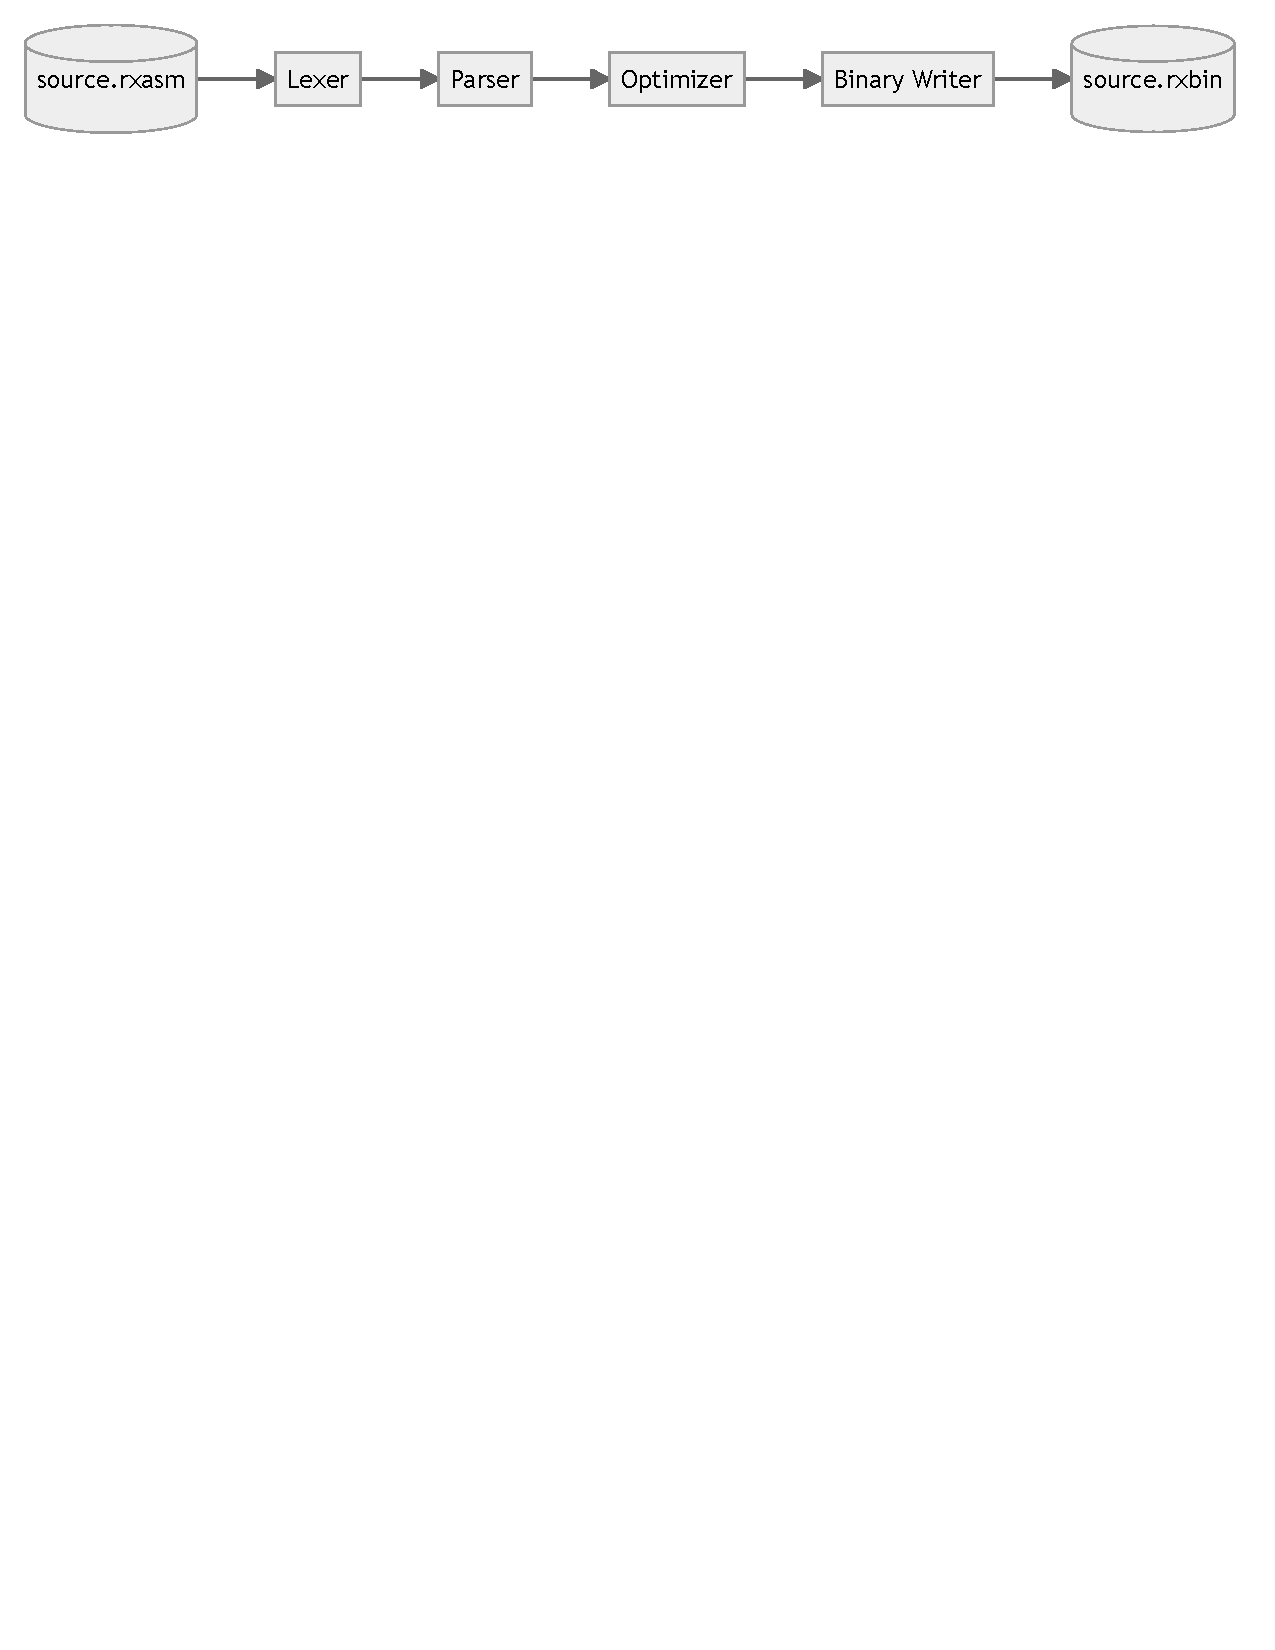
\includegraphics[width=\textwidth]{charts/asmstructure.pdf}

% \end{wrapfigure}
The assembler processing goes through a number of steps in a single
pass: first, the Lexer / Scanner tokenises the RXAS code. After that,
the Parser parses the structure into a series of instructions. The
binary writer generates the binary code and constant pool for the
program at hand. The backpatcher runs last and handles forward references.

\section{Input/Output}

The \code{rxas} assembler has a \code{.rxas} file as input and
produces an \code{rxbin} file as output, which can be considered an
\emph{object module}, as it has unresolved addresses, which can be
resolved by the linkage editor component of the \code{rxvm} virtual
machine interpreter. It also produces a report to stdout (in case of
errors only) and can produce a trace file in Debug/verbose mode
(option \code{-d}).

\section{Character sets}
The input file is assumed to be valid UTF8.
The assembler, like the compiler, operates using two character
sets. The first is for symbols in the assembler language
statements. These are all composed of the ASCII subset of Unicode. The
second character set is used for data; the contents of
variables. Here the whole of Unicode can be used.

\section{Command Line Arguments}
When the command line argument -h is specified the options are shown:\\
\fontspec{IBM Plex Mono}
\begin{shaded}
  \small
  \obeylines \splice{rxas -h | sed "s/&/\and/g"}
 \end{shaded}
 \fontspec{TeX Gyre Pagella}

\section{Optimizer}
The assembler contains an optimizer; this is different from the
optimizer which is part of the compiler. This phase of the assembler
is running always, except when switched off by the \code{-n}
options. When there is any doubt whether any encountered problem is
caused by the optimizer, switching it off can help diagnosing the problem.

\section{Assembler Directives}
For machine instructions, see the \emph{\crexx{} VM
  Specification}. This section discusses instructions to the
assembler, which are called \emph{directives} to clearly distinguish
them from virtual machine instructions. These are necessary to pass information into the compiled
\emph{.rxbin} binary file, to enable execution by the \emph{rxvm}
virtual machine. In the following itemized list, \emph{italic}
descriptors are categories, while items in roman type are literal directives.
\begin{description}
\item[\emph{comments}] A block comment can be made by
  surrounding the text block with \code{/*} and \code{*/}
  indicators. The \code{*} (asterisk) can be used as a line
  comment. The remainder of the line after a line comment is ignored.
\item[\emph{labels}] A label (a string ending with a colon, indicated in the machine
  instructions documentation as an \code{ID}, is a target for
  branching-type instructions.
  Example:
  \begin{lstlisting}[language=rxas]
loop:
    fndnblnk r3,r1,r3   /* find first/next non blank offset    */
    ilt r5,r3,0         /* if <0, nothing found, end search    */
    brt break,r5
    inc r6              /* else increase word count            */
                        /* offset of word is in R3             */
    copy r8,r3          /* save offset of word                 */
    fndblnk r3,r1,r3    /* from offset find next blank offset  */
    ieq r7,r6,r2        /* is this the word we are looking for?*/
    brt wordf,r7        /* go and fetch it                     */
    ilt r5,r3,0         /* if <0, nothing found, end search    */
    brt break,r5        /* word not found                      */
    bct loop,r4,r3      /* continue to look for next non blank char */
  \end{lstlisting}
\item[\emph{registers}] \code{r0 ...\emph{n}} are names of registers, indicated
  in the machine instructions documentation as \code{REG}.
\item[.globals=\{INT\}]Defines \emph{int} global variable \code{g0 ... g\emph{n}}. These can be used within any procedure in the file.
\item[.locals=\{INT\}] The number of local registers (local to the
  source program). This number needs to be 1 greater than the highest
  used register number.
\item[.expose=\{ID\}]Any global register marked as exposed is available to any file which also has the corresponding exposed index/name.
\item[.src] Used to document source lines. This is an optional
  directive that is added for every source line processed by the
  \code{rxc} compiler. It is used for TRACE and SOURCELINE.
\item[.proc] A procedure is a scope delimiting mechanism for the access of
  registers. The registers of a procedure are independent of the
  caller's registers. The VM maps its registers to the registers in
  the caller. Each time a procedure/function is called a new \emph{stack frame} is provided. This means that the called function has its own set of registers.
The function header defines how many registers (called locals) the
function can access - for practical purposes one can consider that any
number of registers can be assigned to a function. In addition, each file defines a number of global registers that can be shared between procedures.

\end{description}
\section{Examples}
Here are several examples of how to use \code{rxas} to
assemble a program into an object module.

\section{In-line assembly}\label{inlineAssembly}
The \crexx{} compiler \emph{rxc} enables\footnote{When used with
  \code{options level b}} inline assembly through the
\textbf{assembler} statement. When used in this way, a lot of
the complications of an assembly language program can be handled by the
\crexx{} compiler, like assigning registers to variables, and the
conversion of datatypes like \emph{integer} for display as \emph{string}.

\lstinputlisting[language=rexx,label=iexample,caption=ipowexample]{examples/pow.rexx}
\fontspec{IBM Plex Mono}
\begin{shaded}
  \small
\splice{rxc examples/pow} \obeylines
\splice{rxas examples/pow} \obeylines \splice{rxvm examples/pow}
 \end{shaded}
\fontspec{TeX Gyre Pagella}

This is a simple and straightforward way to complement the low level
assembler instructions with the power of the \textsc{Rexx}
language. The following example intends to explain how this is
implemented; it can be skipped without consequences.

In this example, the compiler generates the following assembler source:
\lstinputlisting[language=rxas,label=ipow_rxas_example,caption=ipow
rxas example.]{examples/pow.rxas}

The \code{.src} directives (intended for trace and sourceline) indicate where the work is done. The
variables are assigned, as integers, to the registers \code{r1} and
\code{r2}. The line \code{ipow, number, power} becomes \code{ipow
  r3,r1,r2}, and the display on the terminal is handled by the
\code{itos},\code{sconcat} and \code{say} instructions.

This is an example, with the remark that in this case, the microcode
for \code{ipow} is always executed, the example in \textsc{crexx} on
page \pageref{fpowexample} shows that the \crexx{} optimizer of the
compiler can eliminate this code entirely.

The use of Assembler Directives is not allowed in inline assembly, so
(as an example) is it not possible to define procedures in an inline
assembler block.

\section{Troubleshooting}
The assembler will give messages when there are problems in a source
file. These are hopefully of enough clarity to resolve the immediate
problem with syntactic issues or typos. When a program assembles
correctly but its behaviour is unexpected, or its output is incorrect,
a number of different strategies can be followed.

\subsection{Adding say statements}
It is easy to add \code{say} statements to your program. Unlike
\textsc{Rexx}, there is no trace statement for assembler programs. It
is possible to disassemble (see page \pageref{disassembler} an \code{.rxbin} module, and reassemble it
with added statements.

\subsection{Using the debugger}
The \code{rxdb} debugger has a mode for assembler. This can be used to
set breakpoints and/or step through the code; here the registers can
be traced so variables in your program can be followed and the
comparisons and branches can be checked. For more information about the
debugger, see page \pageref{debugger}.


\section{Reference}

\chapter{\crexx{} Disassembler}\label{disassembler}
A disassembler reverses the actions of an assembler; where the
assembler turns a text file containing unstrictions and directives
into a binary executable, the disassembler returns this binary file
into its text form\footnote{as much as possible, given the fact that
  some information on literals has disappeared};in this case it
delivers a disassembly which in itself can be re-assembled - and still
works. 

\section{Input/Output}

The \code{rxdas} disassembler has a \code{.rxbin} file as input and
produces a text file as output which goes to \code{stdout}. In this
text file a disassembly has taken place; labels are synthetic and
based on the combination of instructions around them. As clearly can
be seen in the above, the labels generated by the \crexx{} compiler
are not the same as the ones generated by the disassembler. With
option \code{-p}, the constant pool of the \code{.rxbin} file is
printed first, before the rest of the disassembly. 

\section{Command Line Arguments}
When the command line argument -h is specified the options are shown:\\
\fontspec{IBM Plex Mono}
\begin{shaded}
  \small
  \obeylines \splice{rxdas -h | sed "s/&/\and/g"}
 \end{shaded}
 \fontspec{TeX Gyre Pagella}

 \section{Example}
 \lstinputlisting[language=rexx,label=disasm,caption=disasmexample]{examples/sumLoop1000.rexx}
 % \splice{rxc examples/sumLoop1000} \obeylines
 \lstinputlisting[language=rxas,label=disasm1,caption=disasmexample1]{examples/sumLoop1000.rxas}
 \splice{rxas examples/sumLoop1000}
This program contains the generated assembler as the \code{rxc}
produces it from the \textsc{Rexx} source. What follows is the
disassembly from the assembled \code{.rxbin'} file.
 % \begin{figure}[p]
 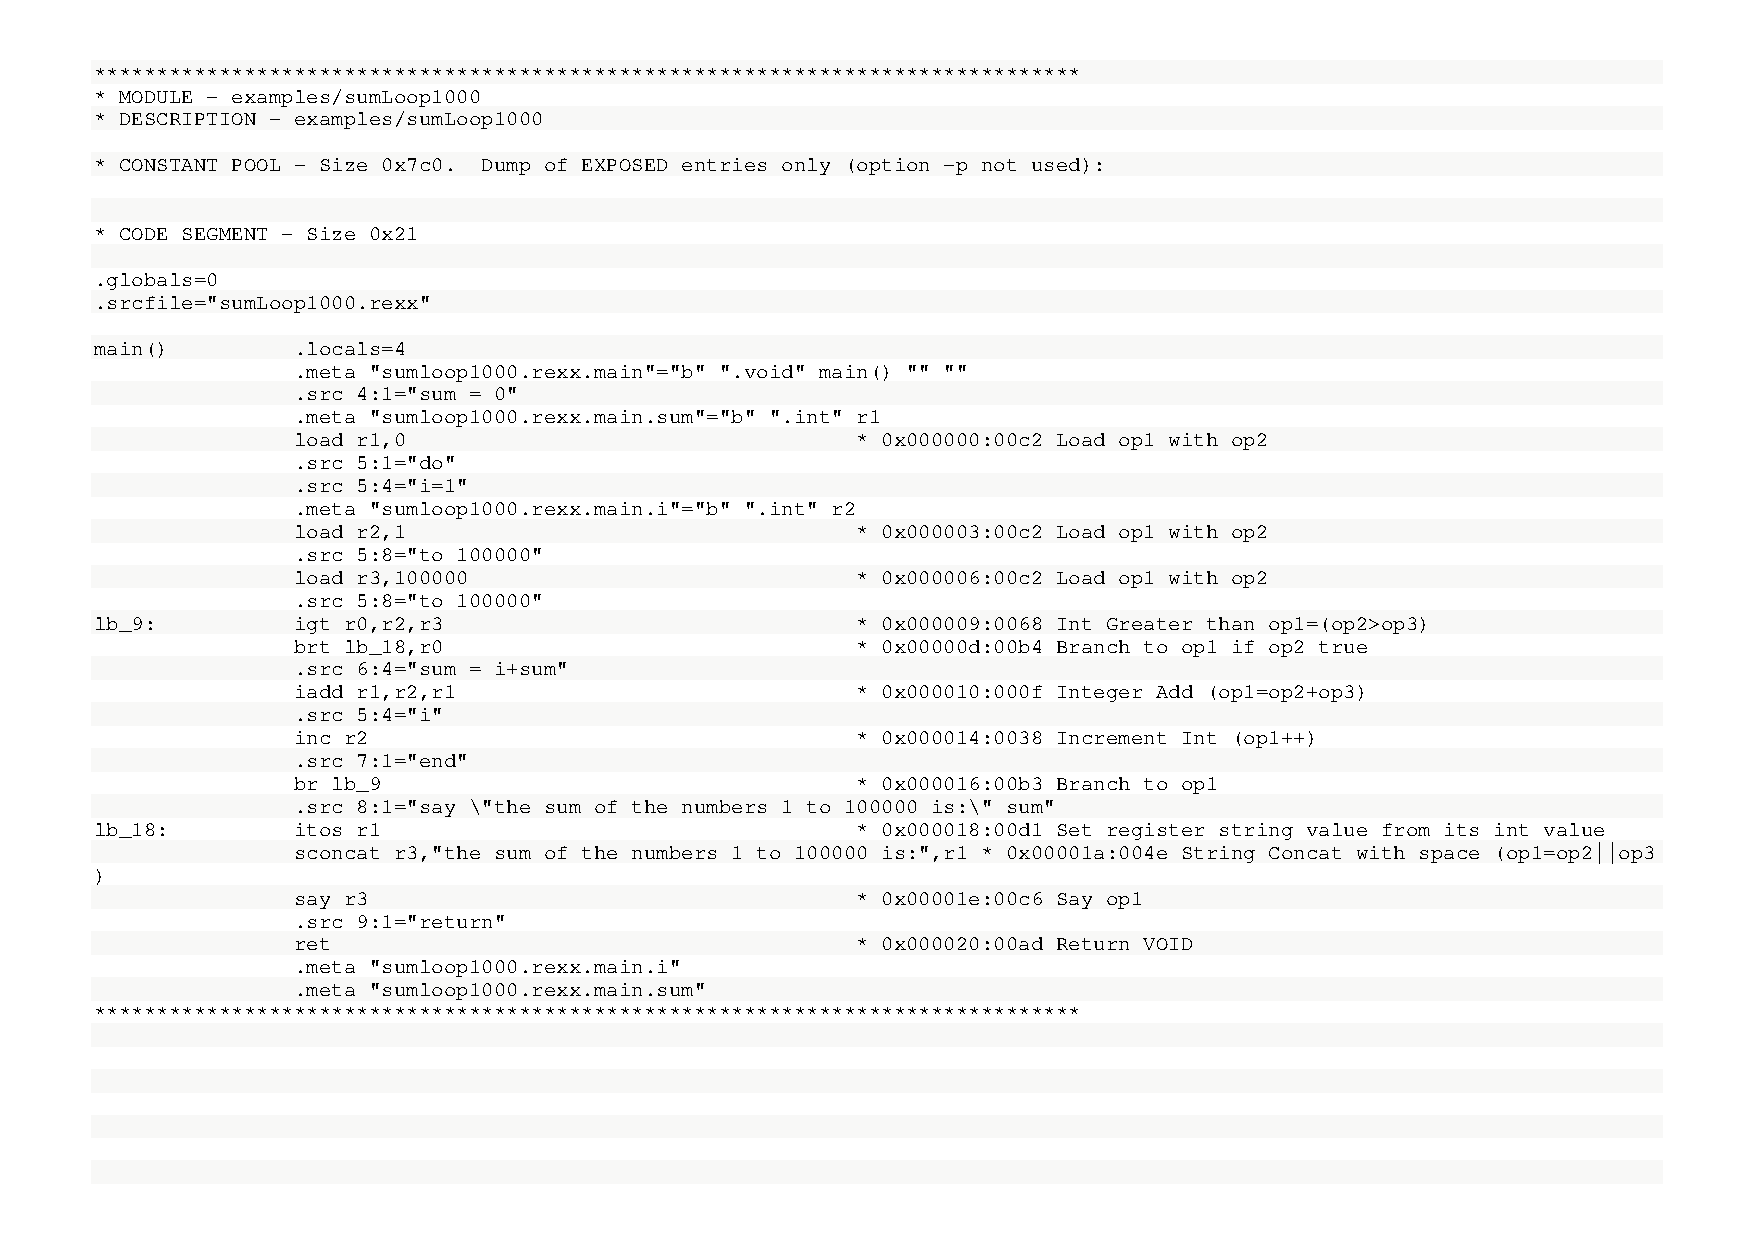
\includepdf{examples/disasm.pdf}
 % \caption{The output of a disassembly.}
%   \label{fig:disasm}
% \end{figure}

\fussy
 \subsection{Remarks}
 The zebra fanfold has the output of the disassembler; the procedure name,
 \code{main}, is identical, but the first label generated by the
 compiler, \code{l7dostart:} is called \code{lb_9} in the disassembler
 output. This is of no consequence for a subsequent re-assembly and
 execution of the program.

 The instructions can be different due to the optimizations the
 assembler performs. When the compiler has performed optimizations,
 this is already visible in the \code{.rxas} file.

Also, the disassembler affixes the standard instruction documentation,
which is the same as generated by \code{rxas -i}, in a line comment
after the instructions. 
 
 When stepping through a program using the \crexx{} Debugger (which is
 mentioned in the next chapter), the disassembly is the most
 representative record of what is in the \code{.rxbin} executable. 

\chapter{\crexx{} Debugger}\label{debugger}
The debugger is the only program in the toolchain delivered with \textsc{Rexx}
as its source code; the other programs, at the moment, are compiled
from C. It is easily adaptable and can be regarded a \emph{debugger
  construction set}. By adapting and recompiling the user can
implement their own wishes for a debugger. In this sense, it can be
seen as an open-ended complement to the \textsc{Rexx} \code{trace}
statement. Because it has modes for \textsc{Rexx} as well as
\code{rxas} Assembler, it is a very useful tool for debugging
low-level problems.
\section{Command Line Options}
\fontspec{IBM Plex Mono}
\begin{shaded}
  \small
  \obeylines \splice{rxdb -h | sed "s/&/\and/g"}
 \end{shaded}
\fontspec{TeX Gyre Pagella}
\section{Runtime Options}
After the \code{rxdb} program is started, a few runtime options appear in the
delivered version. This is an example session:
\chapter{\crexx{} C Packer}
The C Packer program converts the \emph{.rxbin} files into a C
language structure which links together all needed modules, and a
large part of the Virtual Machine infrastructure, which file then can
be compiled and link edited by the C compiler. GCC and Clang are the
targeted compiler toolchains for Linux, macOS and Windows.
\section{Command Line Options}
\fontspec{IBM Plex Mono}
\begin{shaded}
  \small
  \obeylines \splice{rxcpack -h | sed "s/&/\and/g"}
 \end{shaded}
\fontspec{TeX Gyre Pagella}


\backmatter
\listoftables
%\listoffigures
%\lstlistoflistings
\printindex
\clearpage
\psset{unit=1in}
\begin{pspicture}(3.5,1in)
  \psbarcode{\isbn}{includetext guardwhitespace}{isbn}
\end{pspicture}
\end{document}
